\section{Results}

\subsection{Comparison of Performance}
We measure performance of the different systems as average traffic flow
$[\unit{vehicles/h}]$ as a function of average traffic density
$[\unit{vehicles/km}]$. The speed limit was fixed to $50 \unit{km/h}$ in all
experiments. Data is presented in fig \ref{performace}.\\\\

Initially, the performance of all three systems grow linearly as traffic is
light enough to allow all cars to keep maximum allowed speed. As traffic grows
denser, the cars have to slow down to keep constant time headway. All three
system follow the same performance curve until a density of $50.0
\unit{vehicles/km}$ is reached. At this point, phantom jams appear in the
\emph{normal driver} system and traffic flow drops dramatically. For the
\emph{Adaptive Cruise Control} system and the \emph{Enhanced Adaptive Cruise
Control} system, phantom jams were first observed at $56.3 \unit{vehicles/km}$
and $68.8 \unit{vehicles/km}$ respectively. Fig \ref{performance} also shows
that the performance of these two systems is not reduced by the phantom jams
as severely as for the \emph{normal driver}.

\begin{figure}[h!]
    \begin{center}
    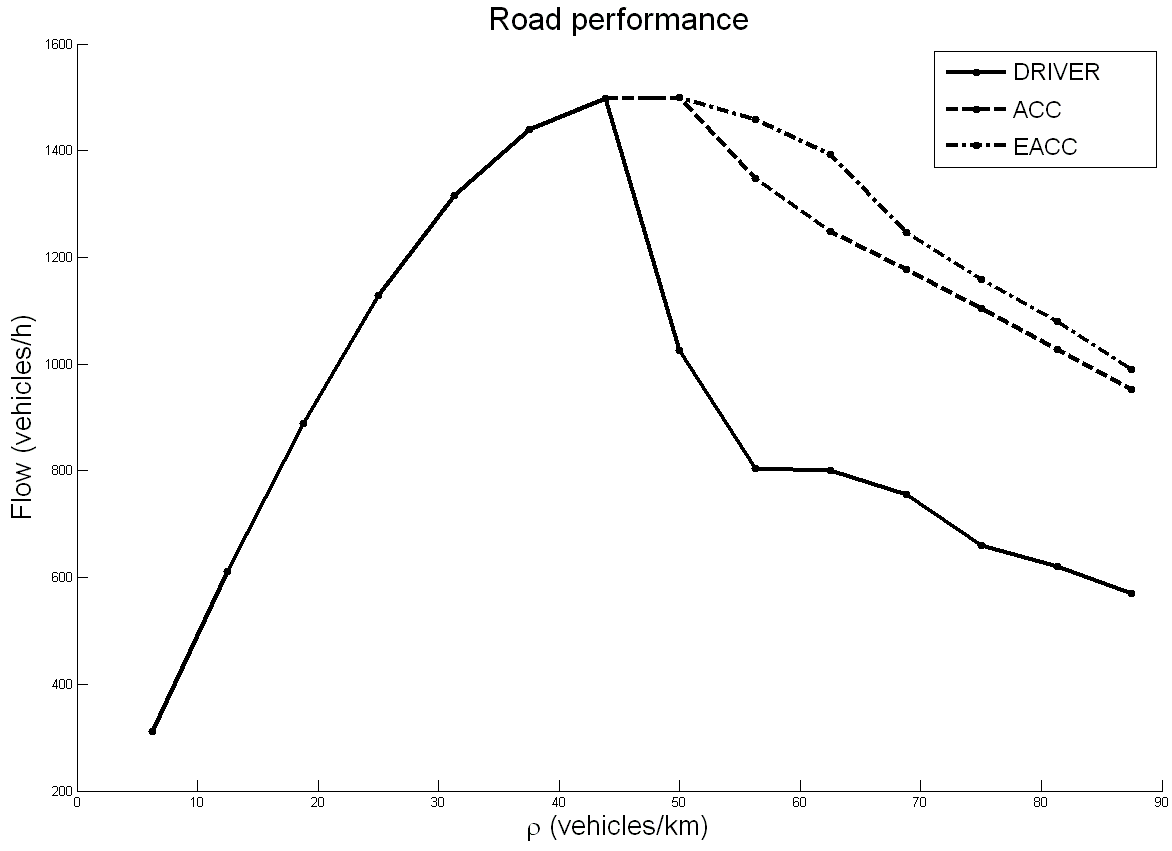
\includegraphics[width=0.8\textwidth]{flowdensity_2.png}
    \caption{\label{performance}
Traffic flow as a function of traffic density. Data from simulator.
$RoadLength=800 \unit{m}$, $SpeedLimit=50 \unit{km/h}$, $TimeHeadway=1.5
\unit{s}$. Traffic flow was measured when traffic conditions had stabilized.}
    \end{center}
\end{figure}


